\subsection{Stepper \hfill IP}
\begin{footnotesize}
    \begin{center}
        \begin{minipage}{0.4\linewidth}
            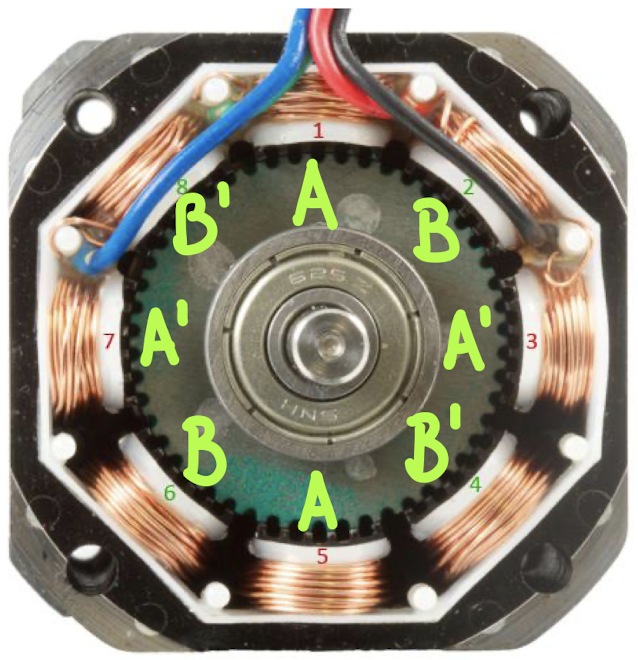
\includegraphics[width = 0.6\linewidth]{src/images/MAEIP_Stepper}
        \end{minipage}
        \begin{minipage}{0.58\linewidth}
            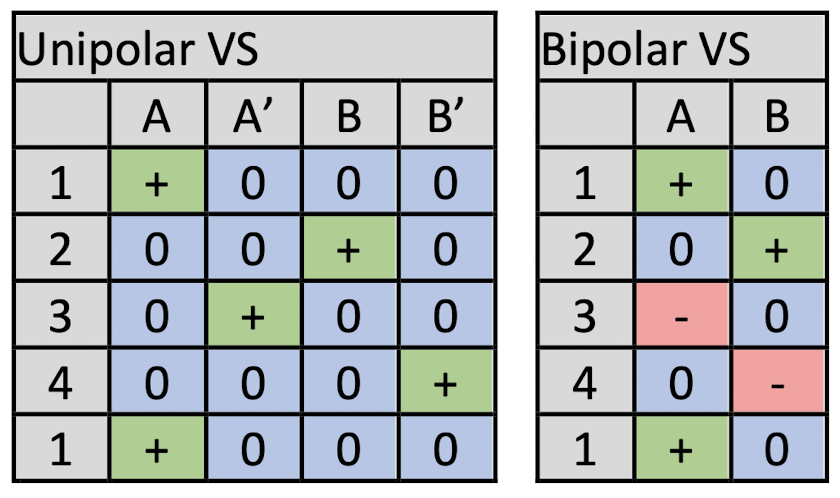
\includegraphics[width = 0.8\linewidth]{src/images/MAEIP_Stepper_Tab1}
        \end{minipage}
        \begin{minipage}{0.4\linewidth}
            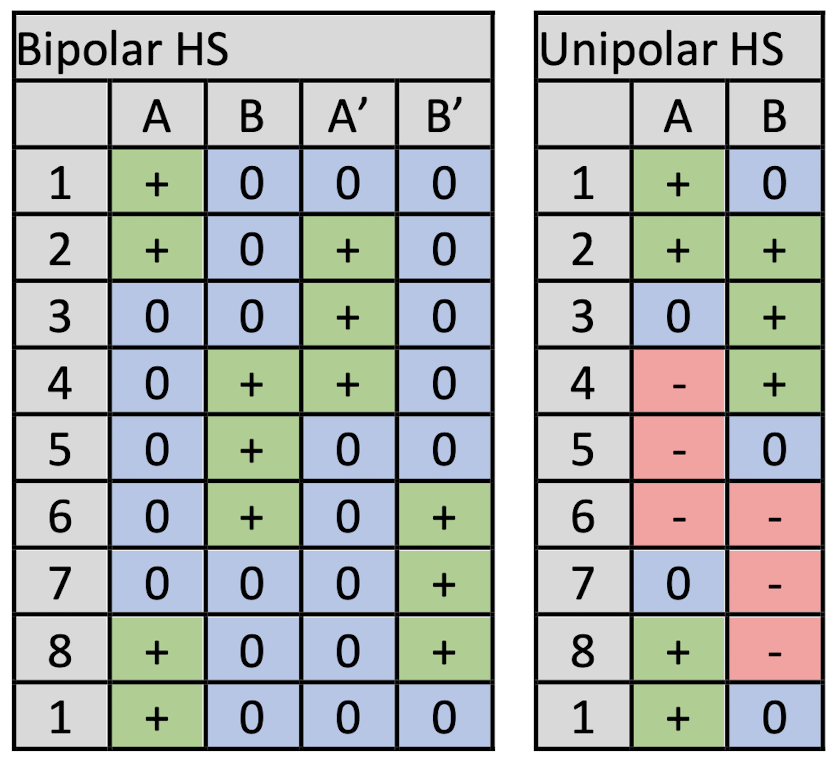
\includegraphics[width = 0.8\linewidth]{src/images/MAEIP_Stepper_Tab2}
        \end{minipage}
        \begin{minipage}{0.58\linewidth}
            \begin{empheq}[box=\fbox]{align*}
               \alpha &= \frac{360^\circ}{z \cdot p}  \quad  \mid \quad n = \frac{\alpha}{360^\circ} \cdot f 
               \\\alpha &= \text{Schrittwinkel (Vollschritt)}
               \\z &= \text{Zähnezahl Polscheiben}
               \\p &= \text{\# Spulenpaare}
               \\f &= \text{Pulsfrequenz}
            \end{empheq}
        \end{minipage}
    \end{center}
    \begin{scriptsize}
        \begin{itemize}
            \item \textbf{Unipolarer Vollschritt:} 
            \\zuletzt bestromtes Spulenpaar aus / benachbartes Spulenpaar ein
            \item \textbf{Unipolarer Halbschritt:}
            \\zuletzt bestromtes Spulenpaar bleibt / benachbartes Spulenpaar wechselt \\Schaltzustand
            \item \textbf{Bipolarer Vollschritt:} 
            \\zuletzt bestromte Spulenpaare aus / benachbarte Spulenpaare ein (!Mehrzahl!)
            \item \textbf{Bipolarer Halbschritt:}
            \\zuletzt bestromtes Spulenpaar bleibt (z.B. A und A') / benachbartes Spulenpaar \\wechselt Schaltzustand (z.B. B und B')
        \end{itemize}
    \end{scriptsize}
\end{footnotesize}
\cbreak